\documentclass{article}

\title{11123Measuring Red Algae in the Santa Ana River}
\author{EA30: Valeria Sanchez, Frank Lyles, Olivia Howie} 

\usepackage{Sweave}
\begin{document}
\Sconcordance{concordance:Tuesday_1_Report_Outline.tex:Tuesday_1_Report_Outline.Rnw:%
1 81 1 49 0 4 1 4 0 6 1 27 0 14 1 6 0 6 1 6 0 4 1 6 0 4 1 6 0 19 1}



\maketitle

\newpage
\tableofcontents
\newpage

\section{Introduction}


\subsection{Problem Statement}

The abundance of red algae, or as it is known by its scientific name Rhodophyta, has recently risen significantly in the Santa Ana River, at a questionably similar time that the Santa Ana Sucker, an endangered fish in the river, has been experiencing population declines. This experiment explores the change in red algae (Rhodophyta) presence in the Santa Ana River and the possible relationship it holds with Santa Ana Sucker's decline. Using measurments of river water temperature, overhead tree canopy cover, and sediment type we explore the connection these aspects of the river and their relationship with the red algae.

\subsection{Background Research} 
This project is motivated by the decline of the threatened Santa Ana sucker, a small freshwater sucker fish endemic to southern California, where it is now present in only three rivers. While there are several threats to the Santa Ana sucker, including fragmentation of its river habitats and decreasing water levels and degradation to the riparian vegetation along the river (Thomson 2010), red algae presence has significantly increased at this same time that the Suckers are dying. For the Santa Ana River sucker habitat, a central threat is the invasive Red Algae that has been spreading with alacrity in areas where the fish are known to be, including the reach below the Rapid Infiltration and Extraction (RIX) Treatment plan (Los Huertos 2016).There are concerns that it may be one of the contributing factors to the suckers decline. This project therefore focuses on qualitatively identifying and analyzing the substrate on which the red algae grows, because one of the aspects of the suckers habitat is the presence of coarse substrate, that is, gravel and cobble, as opposed to silt and sand (Thomson et al. 2010, 321). The sucker has adapted to feeding on the diatoms that tend to grow on the former. There is also evidence that some of the diatoms on which the sucker feeds may be able to grow on the algae (are epiphytic) (Los Huertos 2016). This may lead to the sucker being in contact with the algae when feeding. If the sucker is ingesting the algae, this may constitute a factor to the Suckers decline. Of course, ingesting the algae is not a necessity to the fish being negatively impacted; the algae may also disrupt the fishs well-being in unknown ways. Some researchers suggest that it actually crowds out the diatoms on which, along with algae and detritus, the sucker feeds (Thomson 2010, 322). The presence of the algae in the same area and on the same type of substrate as the fish could indicate competition for resources between the algae and the fish.'

\subsection{Objectives}
Our objective for this project is to unveil (even if just a little!) the possible relations that red algae has in the Santa Ana River. Our goal is to uncover the question "where does the red algae occur?" and relate it to the possible factors of canopy cover, temperature, pebble count. Our research is a tool to be developed, used, re-used, re-created, or whatever need be for fellow researchers who are interested in this connection as well. 

\subsection{Materials and Equipment} 
GPS Spherical Canopy Densiometer, 30cm x 30cm PCV Quadrat, Analog Thermometer, 10 m string/rope, Recording material, Computer, RStudio Server, Microsoft Excel

\section{Methods}


\subsection{Site Description}
<<<<<<< HEAD

FIX SITE NAMES
We evaluated 3 reaches of the Santa Ana River, with 9 observations per reach. Site A (plunge pool): 34*2’5” N, 117*21’17” W Site B (below confluence): 34*2’21” N, 117*21’20” W Site C (above confluence): 34*2’29” N, 117*21’15” W. Each observation contains the following variables: algae percent cover, canopy cover, water temperature, bed composition. near Colton, California (Figure \ref{SAR_Image}). 
=======
This data was collected in the Rialto portion of the Santa Ana river for locations 2, 3, and 4. Site 4 was the plunge pool, located the furthest downstream. Site 3 was below the confluence and Site 2 was upstream from the confluence. 
We evaluated 3 reaches of the Santa Ana River, with 9 observations per reach. Site 4 (plunge pool): 34*2’5” N, 117*21’17” W Site 3 (below confluence): 34*2’21” N, 117*21’20” W Site 2 (above confluence): 34*2’29” N, 117*21’15” W. Each observation contains the following variables: algae percent cover, canopy cover, water temperature, bed composition. near Colton, California (Figure \ref{SAR_Image}). 
>>>>>>> f52c5f4ece92f8791d64a3fdd4871d215ac726dc

\begin{figure}
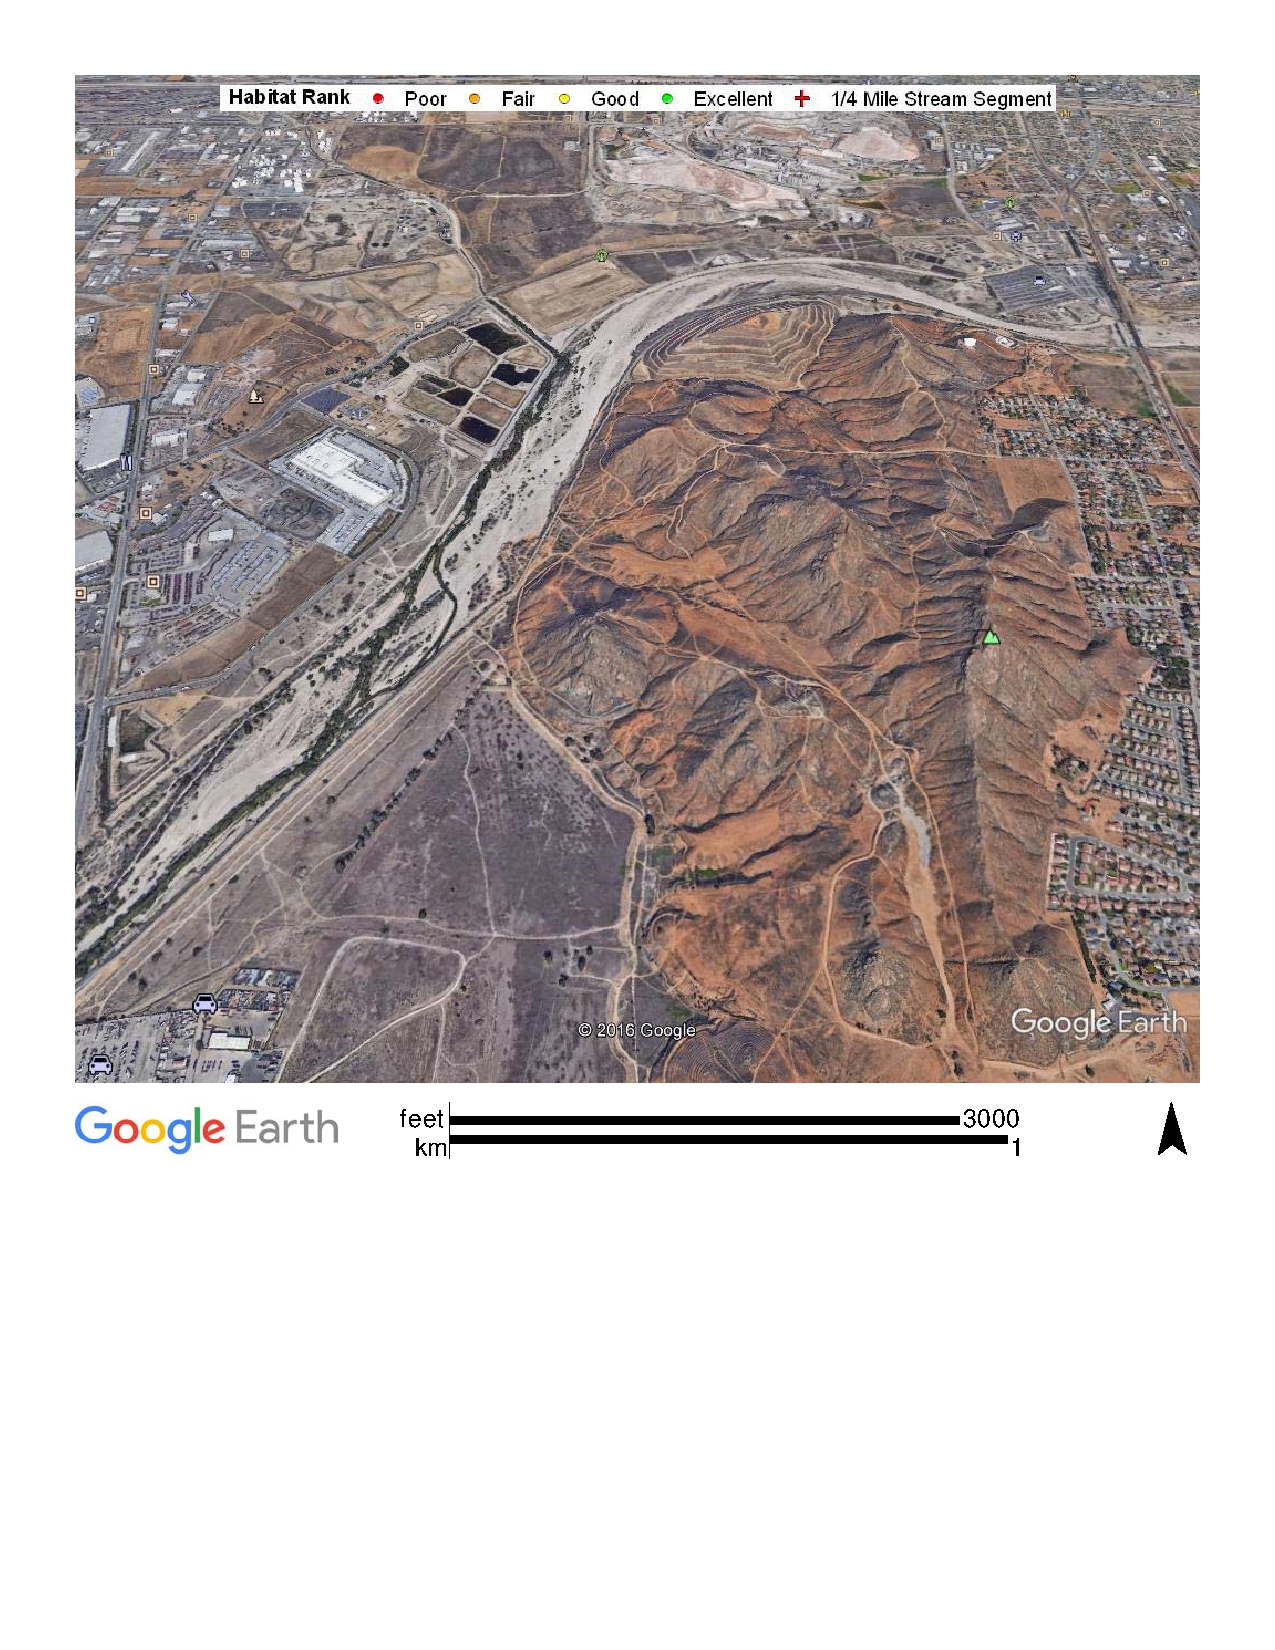
\includegraphics[width=1.00\textwidth]{Figures/SantaAna_SatelliteImage}
\caption{Google Earth --THIS IS HOW YOU DO A CAPTION IN CASE WE NEED IT}
\label{SAR_Image}
\end{figure}

\subsection{Field Methods}
The collection of data on the algae abundance, sediment type, vegetation canopy cover, 
and temperature of the Santa Ana River was done along the section of the river described
in the site description section on September 20th, 2016, from 1pm to 3:30pm.

9 measurements of each parameter were taken at Sites 4, 3, and 2, for a total of 27 measurements. 
At each site, beginning at Site 4, the following procedures were followed: 
A spot was chosen along the right bank. Each of the parameters were then measured.
For estimating algae abundance, we placed the 30  x 30 cm quadrat above the river bed and estimated
the percent that was covered by algae to the nearest 10 percent.

The sediment type of the site was characterized as either fine or coarse based on the grain size of the 30x30cm section of stream bed covered by the quadrat as either fine or coarse. Coarse substrate was classified as anything larger than pebbles or sand, that is, larger than 6.5cm. If more than half of the area covered by the quadrat was coarse substrate, or fine substrate, the area was characterized as such respectively.

Canopy cover was measured from the same position as the algae by holding spherical canopy densiometer above water at elbow’s length. Based on how many of the 15 intersections on the densiometer reflected overhead canopy, cover was then quantified on a 0-15 scale, 0 being the no canopy cover and 15 being full cover.

To measure temperature, we submerged the analog thermometer underwater and recorded the temperature in degrees Celsius.

Qualitative aspects of the river, such as presence of a pool or of logs, were also noted at each measurement spot.

Each measurement was then also taken at the middle of the river and the left bank of the cross-section. 

Steps 1)-7) Were repeated at two cross-sections between 0 and 10 meters downstream both chosen using a random number generator for a total of 3 cross-sections along a possible total length of 20 meters, and 3 measurements at each cross-section, for a total of 9 measurements per site. 


Steps 1)-8) were repeated at each Site, moving upstream from 4 to 2, for a total of 27 measurements of each parameter.


\subsection{Laboratory Methods}

\subsection{Statistical Methods}
<<<<<<< HEAD
After conducting our fieldwork, we imported our data in rstudio and generated summary statistics using the following code: 
\begin{Schunk}
\begin{Sinput}
> updateddata= "/home/CAMPUS/fcl02013/Santa-Ana-Sucker-Recovery/Data/Data_TUES_1/updatedtemps.csv"
> importupdated=read.csv(updateddata)
\end{Sinput}
\end{Schunk}
=======
After conducting our fieldwork, we will enter our data in rstudio. We will produce linear regressions of temperature vs algae abundance. We will producelinear regressions of canopy cover vs algae abundance. We will produce linear regressions of canopy cover vs temperature. We will create ANOVA or t-tests of bed composition vs. algae abundance. We will then analyze our data and write a project report 4-5 pages long with pictures and figures. We should hopefully be able to draw conclusions about canopy cover, temperature, and stream bed compositions effect on algae abundance. In qualitative terms, we will synthesize our results with the fish videography team and state whether our observed relationship between stream conditions and algae abundance matches the frequency of their fish observations.
The following code was used to generate summary statisitics. 
INSERT CODE FOR SUMMARY STATISTICS
>>>>>>> f31b8abefbb905befede6108d156a650b766b1ff

Note that *Temp_x* entries were borrowed with permission from Sophie and Nicole's dataset. We also created a "Site_New" field so that our naming conventions whould be consistant with other teams. We then used rstudio to generate the following descriptive statisitcs:  
linear regression of temperature range vs algae abundance
linear regression of canopy cover vs algae abundance
ANOVA of bed composition vs. algae abundance
ANOVA of site location vs. algae abundance
For each of these statistical comparisons, we tested whether we could reject the null hypothesis, and if yes, discuss the implications of those findings. Our results are summarized in the following section. 

\section{Results}

The temperature data we collected with an analogue thermometer was too coarse to really be useful (Figure \ref{Temp}).
\begin{Schunk}
\begin{Sinput}
> plot(importupdated$Temperature,importupdated$Algae, ylab="Algae Abundance (% cover)",xlab="Temperature (*C)",main ="Temperature as a predictor of Algae Abundance",las=1)
\end{Sinput}
\end{Schunk}
So instead used WED1 team's temperature data. The following is a plot of algae abundance as a function of temperature range (*C) at each site. 
\begin{Schunk}
\begin{Sinput}
> plot(importupdated$Temp_range,importupdated$Algae, ylab="Algae Abundance (% cover)",xlab="Temperature (*C)",main ="Temperature Range as a predictor of Algae Abundance",las=1)
> abline(lm(Algae~Temp_range,importupdated))
\end{Sinput}
\end{Schunk}
While using our temperature data yielded p-value: 0.446, using the other teams's temperature range data yilded p-value: 3.49e-05. There is a strong nonrandom relationship between the range of temperatures a site experiences and the abundance of algae. However, with an Adjusted R-squared of only 0.4826, there are clearly other important variables at work. 


The temperature data suggests... (Figure \ref{Temp}).

\begin{figure}
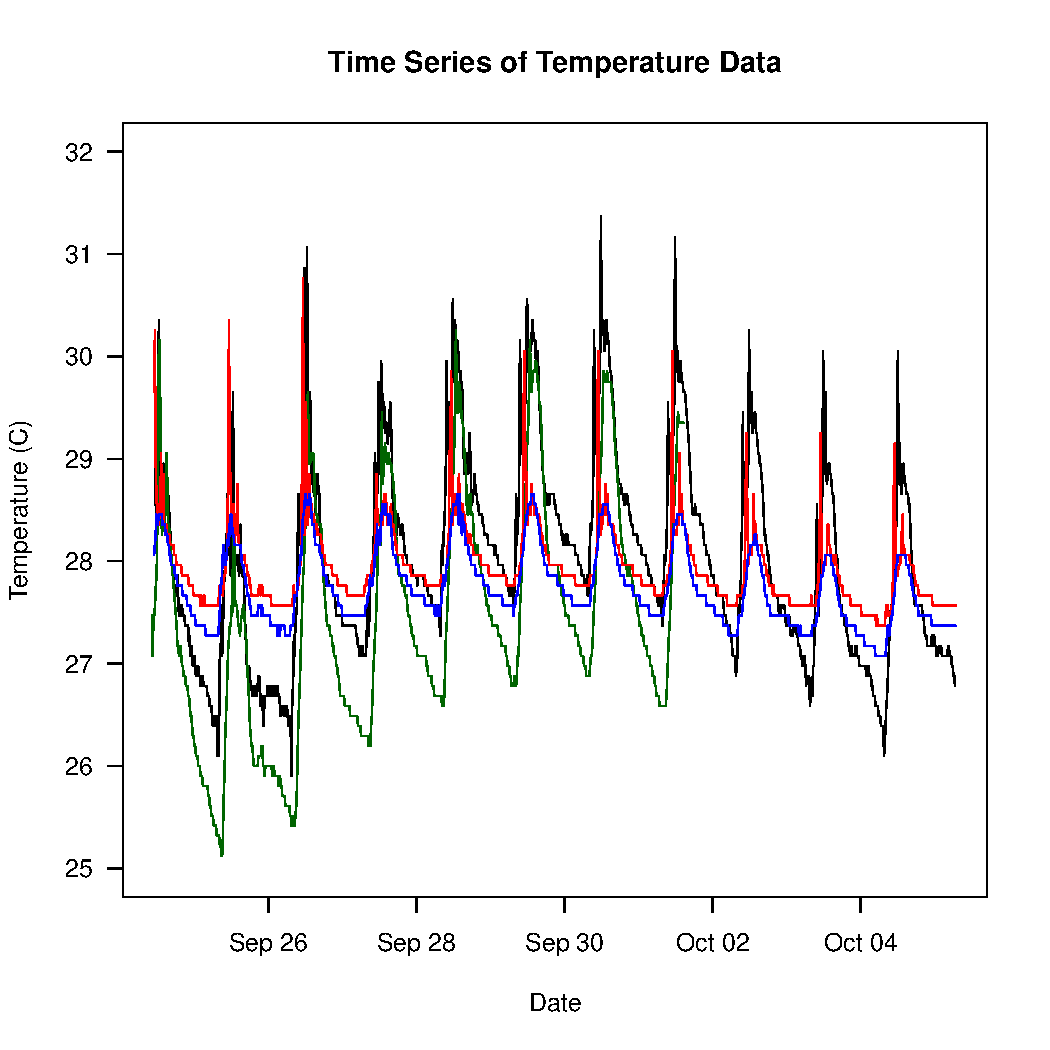
\includegraphics{Figures/Temp}
\caption{Temperature time...}
\label{Temp}
\end{figure}

\section{Discussion}
We

\section{Conclusion and Recommendations}


\end{document}
